\begin{figure}[h]
	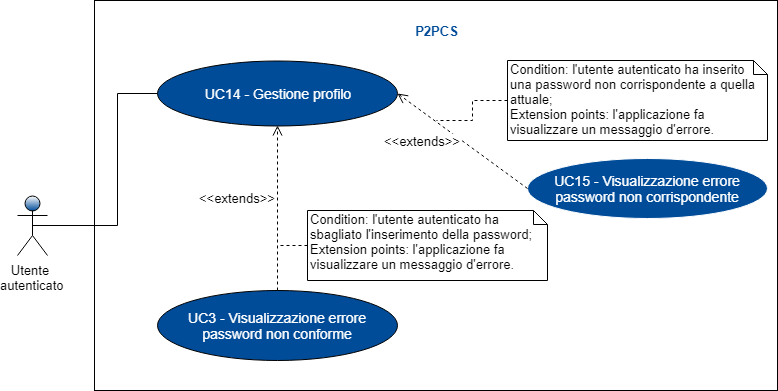
\includegraphics[width=15cm]{res/images/Schemagenerale5.png}
	\centering
	\caption{Schema generale: gestione profilo ed errori annessi}
\end{figure}
\subsubsection{UC14 - Gestione Profilo}
\begin{itemize}
	\item \textbf{Attori Primari}: utente autenticato;
	\item \textbf{Descrizione}: agli utenti autenticati è resa disponibile una maschera che presenta il proprio profilo, dalla quale l'utente può scegliere di modificarlo o eliminarlo;
	\item \textbf{Scenario principale}: l'utente visualizza il profilo e ha la possibilità di: 
	\begin{itemize}
		\item Modifica dati account [UC14.1];
		\item Eliminazione account [UC14.2].
	\end{itemize}
	\item \textbf{Precondizione}: l'utente è in possesso di un account all'interno del sistema. Deve quindi essersi registrato e non aver eliminato l'account;
	\item \textbf{Postcondizione}: l'utente ha effettuato l'operazione di modifica dati oppure l'eliminazione dell'account e il processo è stato confermato dal sistema.
	\item \textbf{Estensioni}:
	\begin{itemize}
		\item Visualizzazione errore email non valida [UC2];
		\item Visualizzazione errore password non conforme [UC3];
		\item Visualizzazione errore password non corrispondente [UC15].
	\end{itemize}
\end{itemize}
\begin{figure}[h]
	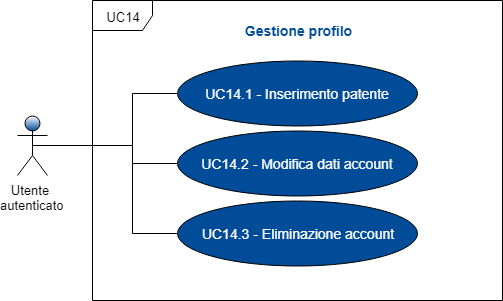
\includegraphics[width=10cm]{res/images/UC14Profilo.png}
	\centering
	\caption{UC14 - Gestione Profilo}
\end{figure} 
\subsubsection{UC14.1 - Modifica dati account}
\begin{itemize}
	\item \textbf{Attori Primari}: utente autenticato;
	\item \textbf{Descrizione}: l'utente ha la possibilità di modificare i propri dati;
	\item \textbf{Scenario principale}: l'utente può modificare:
	\begin{itemize}
		\item Nome [UC14.1.1];
		\item Cognome [UC14.1.2];
		\item Numero telefonico [UC14.1.3];
		\item Email [UC14.1.4];
		\item Data di nascita [UC14.1.5];
		\item Residenza [UC14.1.6];
		\item Password [UC14.1.7].
	\end{itemize}
	e confermare la modifica dei dati [UC14.1.8];
	\item \textbf{Scenari alternativi}: l'utente interrompe la modifica dei dati senza confermare il salvataggio di essi. Il sistema non salverà le modifiche parziali apportate dall'utente me lo riporterà alla schermata di visualizzazione dell'account;	 
	\item \textbf{Precondizione}: l'utente è in possesso di un account all'interno del sistema. Deve quindi essersi registrato e non aver eliminato l'account;
	\item \textbf{Postcondizione}: il sistema ha memorizzato le modifiche apportate ai dati da parte dell’utente;
	\item \textbf{Inclusioni}:
	\begin{itemize}
		\item Inserimento vecchia password [U14.1.7.1];
		\item Inserimento nuova password [UC14.1.7.2].
	\end{itemize}
\end{itemize}
\begin{figure}[h]
	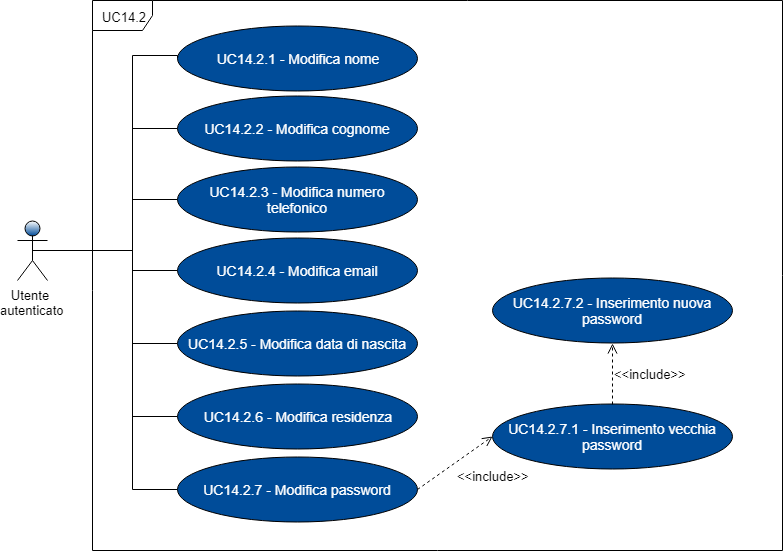
\includegraphics[width=14cm]{res/images/UC14-1Modifica.png}
	\centering
	\caption{UC14.1 - Modifica dati account}
\end{figure}
\newpage 
\subsubsection{UC14.1.1 - Modifica nome}
\begin{itemize}
	\item \textbf{Attori Primari}: utente autenticato;
	\item \textbf{Descrizione}: l'utente ha la possibilità di modificare il nome inserito in precedenza;
	\item \textbf{Precondizione}: il sistema fornisce una schermata nella quale è possibile inserire il nuovo nome;
	\item \textbf{Postcondizione}: l'utente ha inserito il nuovo nome.
\end{itemize}

\subsubsection{UC14.1.2 - Modifica cognome}
\begin{itemize}
	\item \textbf{Attori Primari}: utente autenticato;
	\item \textbf{Descrizione}: l'utente ha la possibilità di modificare il cognome inserito in precedenza;
	\item \textbf{Precondizione}: il sistema fornisce una schermata nella quale è possibile inserire il nuovo cognome;
	\item \textbf{Postcondizione}: l'utente ha inserito il nuovo cognome.
\end{itemize}

\subsubsection{UC14.1.3 - Modifica numero telefonico}
\begin{itemize}
	\item \textbf{Attori Primari}: utente autenticato;
	\item \textbf{Descrizione}: l'utente ha la possibilità di modificare il numero telefonico inserito in precedenza;
	\item \textbf{Precondizione}: il sistema fornisce una schermata nella quale è possibile inserire il nuovo numero telefonico;
	\item \textbf{Postcondizione}: l'utente ha inserito il nuovo numero telefonico.
\end{itemize}

\subsubsection{UC14.1.4 - Modifica email}
\begin{itemize}
	\item \textbf{Attori Primari}: utente autenticato;
	\item \textbf{Descrizione}: l'utente ha la possibilità di modificare l'email inserita in precedenza;
	\item \textbf{Precondizione}: il sistema fornisce una schermata nella quale è possibile inserire la nuova email;
	\item \textbf{Postcondizione}: l'utente ha inserito la nuova email.
\end{itemize}

\subsubsection{UC14.1.5 - Modifica data di nascita}
\begin{itemize}
	\item \textbf{Attori Primari}: utente autenticato;
	\item \textbf{Descrizione}: l'utente ha la possibilità di modificare la data di nascita inserita in precedenza;
	\item \textbf{Precondizione}: il sistema fornisce una schermata nella quale è possibile inserire la nuova data di nascita;
	\item \textbf{Postcondizione}: l'utente ha inserito la nuova data di nascita.
\end{itemize}

\subsubsection{UC14.1.6 - Modifica residenza}
\begin{itemize}
	\item \textbf{Attori Primari}: utente autenticato;
	\item \textbf{Descrizione}: l'utente ha la possibilità di modificare la residenza inserita in precedenza;
	\item \textbf{Precondizione}: il sistema fornisce una schermata nella quale è possibile inserire la nuova residenza;
	\item \textbf{Postcondizione}: l'utente ha inserito la nuova residenza.
\end{itemize}

\subsubsection{UC14.1.7 - Modifica password}
\begin{itemize}
	\item \textbf{Attori Primari}: utente autenticato;
	\item \textbf{Descrizione}: l'utente ha la possibilità di modificare la password inserita in precedenza inserendo prima la vecchia password e poi quella nuova;
	\item \textbf{Scenario principale}: il sistema fornisce per prima cosa all'utente la possibilità di:
		\begin{itemize}
			\item Inserimento vecchia password [UC14.1.7.1].
		\end{itemize}
	e poi di:
		\begin{itemize}
			\item Inserimento nuova password [UC14.1.7.2].
		\end{itemize}
	\item \textbf{Precondizione}: il sistema fornisce una schermata nella quale è possibile inserire la nuova password;
	\item \textbf{Postcondizione}: l'utente ha inserito la nuova password.
\end{itemize}

\subsubsection{UC14.1.7.1 - Inserimento vecchia password}
\begin{itemize}
	\item \textbf{Attori Primari}: utente autenticato;
	\item \textbf{Descrizione}: l'utente deve inserire la password attuale per poterla aggiornare;
	\item \textbf{Precondizione}: il sistema fornisce una schermata nella quale è possibile inserire la vecchia password;
	\item \textbf{Postcondizione}: l'utente ha inserito la vecchia password.
\end{itemize}

\subsubsection{UC14.1.7.2 - Inserimento nuova password}
\begin{itemize}
	\item \textbf{Attori Primari}: utente autenticato;
	\item \textbf{Descrizione}: l'utente deve inserire la nuova password, diversa da quella attuale, per effettuare l'aggiornamento;
	\item \textbf{Precondizione}: il sistema fornisce una schermata nella quale è possibile inserire la nuova password;
	\item \textbf{Postcondizione}: l'utente ha inserito la nuova password.
\end{itemize}

\subsubsection{UC14.1.8 - Conferma modifica dati}
\begin{itemize}
	\item \textbf{Attori Primari}: utente autenticato;
	\item \textbf{Descrizione}: l'utente deve 
	confermare la modifica apportata;
	\item \textbf{Precondizione}: l'utente ha inserito tutti i dati richiesti e desiderati. Si trova dunque davanti ad una schermata con la possibilità di confermare la modifica effettuata;
	\item \textbf{Postcondizione}: l'utente ha confermato di voler rendere effettivo il cambiamento del proprio account.
\end{itemize}

\subsubsection{UC14.2 - Eliminazione account}
\begin{itemize}
	\item \textbf{Attori Primari}: utente autenticato;
	\item \textbf{Descrizione}: all'utente viene fornita la possibilità di eliminare il proprio account e di conseguenza i propri dati all'interno del sistema.
	\item \textbf{Precondizione}: l'utente è in possesso di un account all'interno del sistema. Deve quindi aver effettuato la registrazione e non avere mai effettuato la procedura di eliminazione account.
	\item \textbf{Postcondizione}: l'utente ha cancellato il proprio account e viene riportato alla schermata iniziale dell'applicazione [UC1]. Il sistema non terrà taccia del profilo eliminato.
\end{itemize}

\subsubsection{UC15 - Visualizzazione errore password non corrispondente}
\begin{itemize}
	\item \textbf{Attori Primari}: utente autenticato;
	\item \textbf{Descrizione}: l'utente visualizza un messaggio d'errore in quanto la password digitata in [UC14.1.7.1] non corrisponde alla vecchia password;
	\item \textbf{Scenario principale}: l'utente autenticato cerca di cambiare la password del proprio account;
	\item \textbf{Precondizione}: l'utente autenticato ha inserito una password non corrispondente a quella attuale;
	\item \textbf{Postcondizione}: l'applicazione fa visualizzare un messaggio d'errore.
\end{itemize}



